\chapter{Sampling Time Series Analysis}
In this chapter, a deeper look into the time series is given. Different time series for training and testing purposes are selected and used for the performance of Bayesian inference so that the inferred results can be compared to each other and the measured data. 

\section{Sampling and Testing Time Series Selection}
To set up the analysis, a range of time series that are used for sampling and testing need to be selected. The sampling time series is used on which the Markov chain Monte Carlo algorithms could perform sampling. In other words, the posterior, which is the result of the Markov chain Monte Carlo sampling, is trained based on these data. The generated posterior is then used for Bayesian inference, in which the Monte Carlo simulation is used for random sampling and used as input for the HBV-SASK model. The result generated is then compared with the measured data by visualization so that the differences between the two time series can be observed.

The selection of these times series requires generality, which means that cases of different scenarios need to be taken into consideration. Therefore, a deep look into both datasets provided alongside the HBV-SASK model needs to be conducted. The visualization with times series decomposition is displayed in Figures 3.1 and 3.2. From these visualizations, we figure out that anomalies are integral parts of the entire time series, as they provide valuable information that can be analyzed. These anomalies could be led by different reasons, including climate changes, human activities, and seasonal variations. The predominant reason, however, is flooding~\cite{hbv_sask_anomalies_cause}, which occurs now and then according to the visualizations. They are therefore heavily taken into consideration in terms of sampling and testing times series selection.

For the Oldman Basin, the anomalies are relatively apart from each other. From the trend, we can see that relatively even intervals exist between different occurrences. The entire time series is relatively calm and balanced in comparison to the Banff Basin, indicating the seasons with high levels of discharge and raindrops are more predictable and less extreme. Nevertheless, periods between the years 1992 and 1996 do have higher peaks across the entire times series, with a significant peak presenting in June of 1995. Other small amounts of lower peaks are distributed across the whole time series. The calmness with a certain amount of anomalies makes the Oldman Basin data set an optimal choice for the testing of generality. Therefore, most of the time series that are used for training and testing are selected from the Oldman Basin dataset.

For the Banff Basin, a completely different scenario is presented. High peaks exist everywhere and very often, causing the contrast between the flood period and the drought period to be significant. The data is constantly fluctuating, showing active climate changes and constant floods that are recorded in the area. The trend of the time series also displays no patterns. These characteristics make it an optimal dataset for extreme case prediction, is therefore used for edge cases testing, and has less time series included for testing or training purposes.

To cover the generality of the time series behavior, the following data sets are selected. For training, the following time series are selected:
\begin{itemize}
    \item Short and Calm (Oldman): A short and calm time series. We intend to observe whether the lack of anomalies has an impact on the final inferred result.
    \item Short with Peaks (Oldman): A short time series with peaks that represent potential anomalies. We intend to observe how the small amount of data with extreme anomalies affects the outcome of the Bayesian inference.
    \item Long and Calm (Oldman): A short and calm time series. Alongside the lack of anomalies, the necessity of having a huge amount of data is at the center of the observation.
    \item Long with Peaks (Oldman): A long times series filled with anomalies. This data frame represents the most generality, as it includes both calm periods and anomaly periods.
    \item 97-03 (Oldman): A time frame that lies inside of the Oldman Basin dataset to represent generality. The years correspond to these of the time series "97-03 (Banff)" for ease of comparison.
    \item 97-03 (Banff): A time frame that lies inside of the Banff Basin dataset to represent generality. The years correspond to these of the time series "97-03 (Oldman)" for ease of comparison.
\end{itemize}
For testing, the following time series are selected:
\begin{itemize}
    \item Data containing floods (Oldman): The posterior is tested on a time series where anomalies that represent floods are present. The ability to predict anomalies is tested.
    \item Data displaying calmness (Oldman): The posterior is tested on a calm time series. The ability to cope with calm time regions with less fluctuations is tested.
    \item Banff: A general Banff sub time series with fluctuations that represent the generality of the Banff time series is also used for testing, specifically for the posterior that is trained using the Banff data set.
\end{itemize}

Another important factor for the execution of the HBV-SASK model is the spin-up phase. The spin-up phase is performed before the actual execution of the model, where the model performs execution based on the time series that are in other time frame than the time frame of the actual data, usually a certain period before the period of the actual data. It is performed to ensure the reduction of Initial Condition Bias and temporal consistency~\cite{spin_up_explanation}. A spin-up period of 400 cycles is suggested~\cite{spin_up_explanation}, however, we intend to test the impact of the spin-up phase on efficiency and accuracy metrics, since the lengths of each time series that are used for training are inconsistent. Therefore, 25\%, 50\%, and 100\% of the time, which is the time frame of the actual data, will be tested for the spin-up phase.

\section{Result Interpretation}
After extensive analysis, we conclude that the results of all different training data sets do not show significant differences from each other. The same patterns are shown across all posterior samples from different training data sets. However, there are a few details that show the characteristics of the training data set, which can be observed in the visualizations. In the following paragraphs, the two testing scenarios are interpreted separately. The first four training time series, namely short and calm, short with peaks, long and calm alongside long with peaks are discussed to offer more insights into details, while the rest of the time series are going to be discussed in the next chapter.

For the test case on data containing floods (Oldman), the pattern of all inferred results shows decent performance, particularly regarding trends. The posterior mean aligns well with the measured data, since it closely follows the measured data throughout the entire period, both calm periods and periods with high peaks. This indicates that the algorithm is capable of accurately estimating flood activities and anomalies. On the other hand, the inferred result shows more fluctuations than the measured data, suggesting that the algorithm is sensitive to small changes in the input data or noises.

\begin{figure}[H]
    \centering
    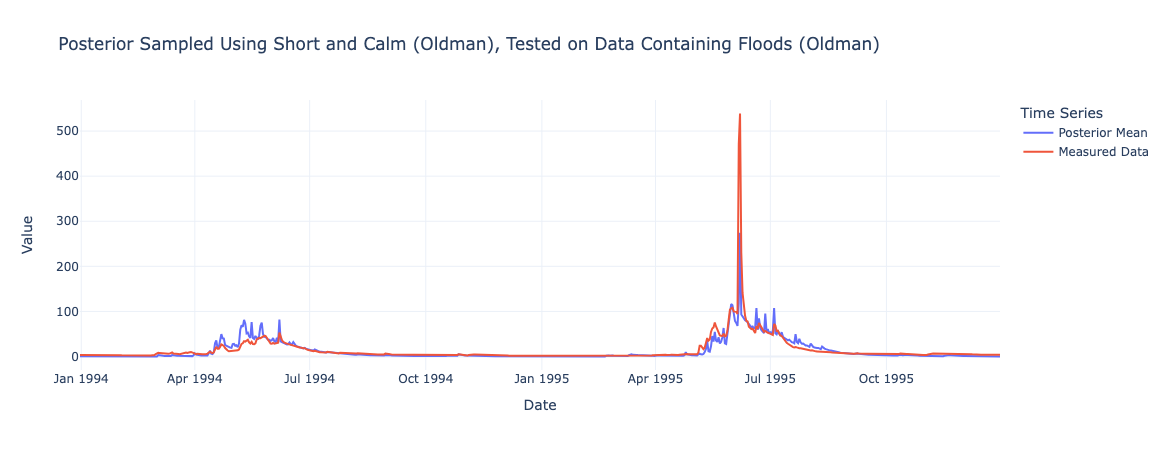
\includegraphics[width=.7\textwidth]{figures/time_series_analysis/ts_int/0_1.png}
    \captionsetup{width=.8\textwidth}
    \caption{The Bayesian inferred result of the posterior sampled using the short and calm time series, testing on data containing floods}
    \label{fig:enter-label}
\end{figure}

\begin{figure}[H]
    \centering
    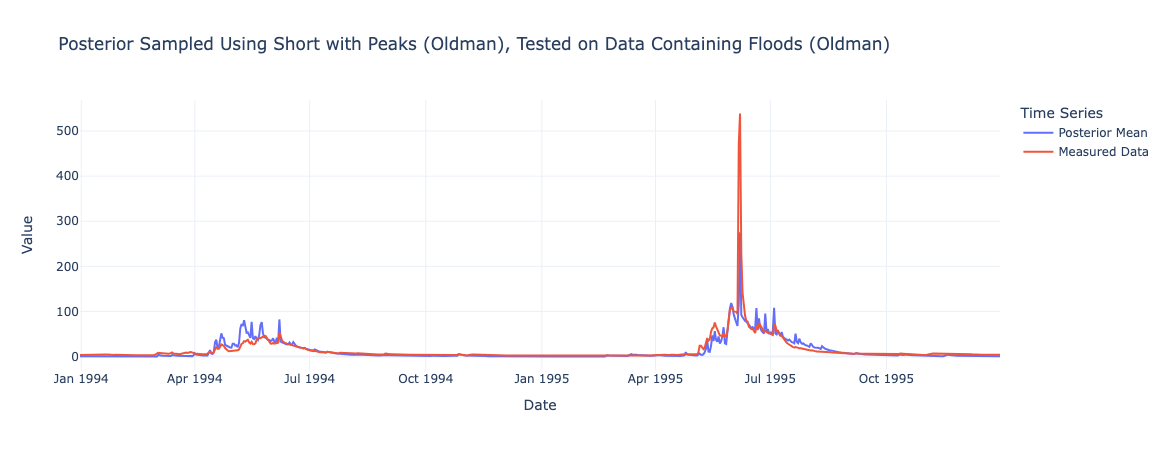
\includegraphics[width=.7\textwidth]{figures/time_series_analysis/ts_int/1_1.png}
    \captionsetup{width=.8\textwidth}
    \caption{The Bayesian inferred result of the posterior sampled using the short with peaks time series, testing on data containing floods}
    \label{fig:enter-label}
\end{figure}

\begin{figure}[H]
    \centering
    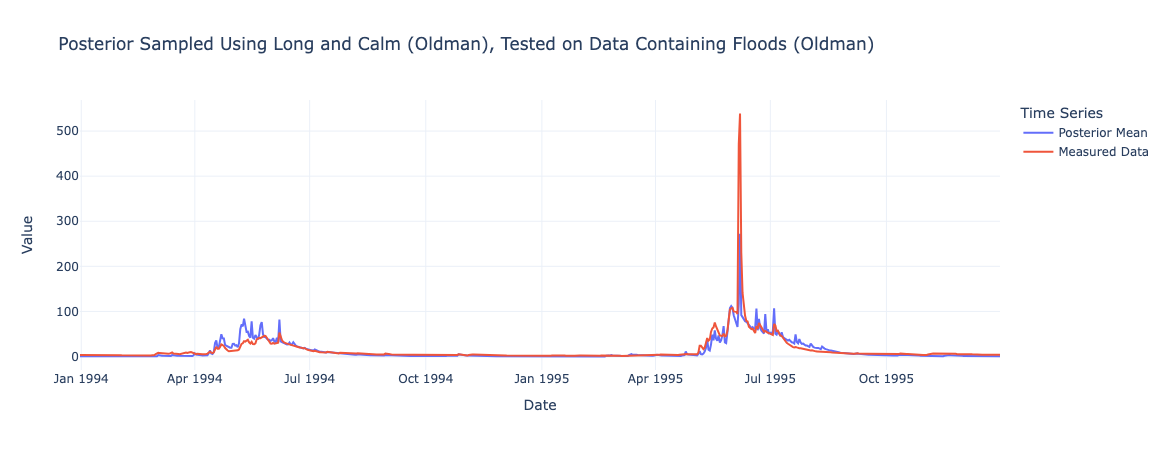
\includegraphics[width=.7\textwidth]{figures/time_series_analysis/ts_int/2_1.png}
    \captionsetup{width=.8\textwidth}
    \caption{The Bayesian inferred result of the posterior sampled using the long and calm time series, testing on data containing floods}
    \label{fig:enter-label}
\end{figure}

\begin{figure}[H]
    \centering
    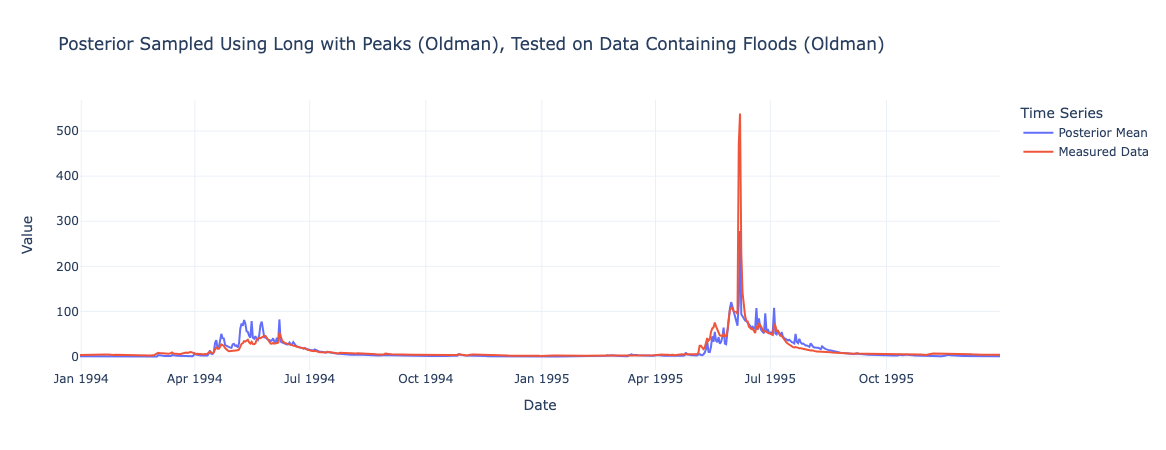
\includegraphics[width=.7\textwidth]{figures/time_series_analysis/ts_int/3_1.png}
    \captionsetup{width=.8\textwidth}
    \caption{The Bayesian inferred result of the posterior sampled using the long with peaks time series, testing on data containing floods}
    \label{fig:enter-label}
\end{figure}

A challenge here is the prediction of the peak in June 1995. The peak indicates a potential strong flood, which is a significant anomaly across the entire time series. For comparison, the exact predicted value is gathered manually from all of these scenarios. These are presented in the table down below.

\begin{center}
\begin{tabular}{@{}lcc@{}}
\toprule
\textbf{Training Data} & \textbf{Short Data Frame} & \textbf{Long Data Frame} \\ \midrule
Calmness           & 272.6607 & 272.9323                  \\
With Peaks             & 275.1849 & 277.3239              \\ \bottomrule
\end{tabular}
\end{center}
The measured result is 539, which is far away from the inferred data. Nevertheless, some level of dependency can be found here, as the training time series with peaks perform better than the ones without peaks. This trend is logical since the posterior sampled from the time series with peaks is more used to anomalies and peaks across the entire time series. On the other hand, the inferred result from the long data frame performs slightly better than the inferred result from the short data frame. This is potentially due to the same reason, where the posterior sampled from the long period might be exposed to more anomalies than the one sampled from the short period. 

For the test case on data displaying calmness (Oldman), more discrepancies are shown in the visualization due to the high scale-in level. The inferred results generally follow the trend of the measured data, especially in the calm periods. In fluctuating periods, the inferred results also fluctuate, with peaks not being predicted as the exact measured value. This high-variable property proves that the algorithm is susceptible to fluctuations, as inferred in the test scenario above. A visualization of the first test case is displayed below. Other scenarios offer similar results to the first test case in terms of visualization and are therefore not presented here. Further comparisons regarding accuracy and efficiency metrics are discussed in the next section, namely result comparison.

\begin{figure}[H]
    \centering
    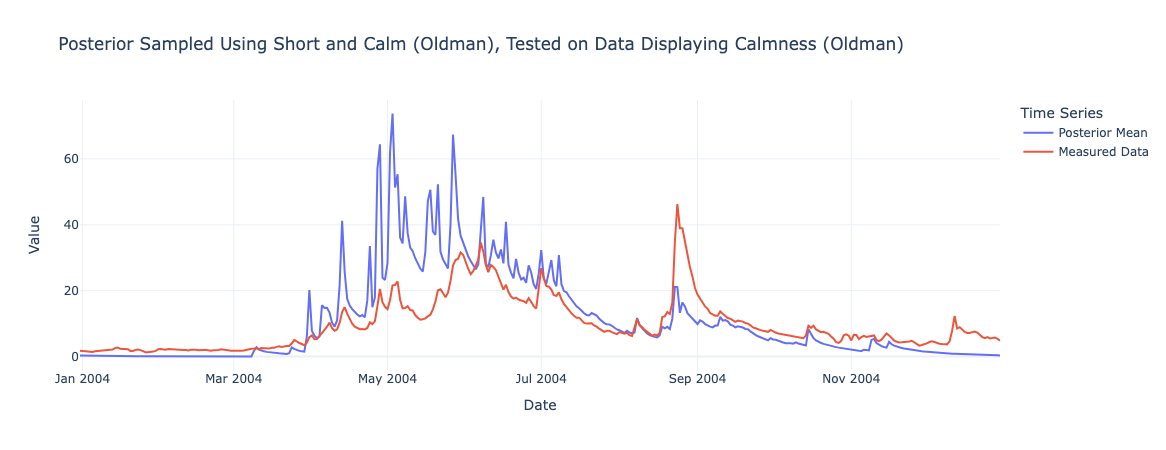
\includegraphics[width=.7\textwidth]{figures/time_series_analysis/ts_int/0_2.png}
    \captionsetup{width=.8\textwidth}
    \caption{The Bayesian inferred result of the posterior sampled using the short and calm time series, testing on data displaying calmness. All of the test cases on data displaying calmness share similar results to this visualization}
    \label{fig:enter-label}
\end{figure}


\section{Result Comparison}
After visualizing the results and comparing them with the measured data, we quantify the accuracy and efficiency using metrics. In the last section, the test mentioned above scenarios will be compared with each other in pairs, so that the dependency between metrics and specific properties of training data sets can be visualized.

The first comparison takes place between the training time series of short periods. The short and calm time series is compared with the short with peaks data frame, so that the factor of including anomalies for the sampling phase of the Markov chain Monte Carlo algorithm is investigated. From the bar chart, the short and calm time series seems to deliver all-around better performance than the training dataset containing peaks. This could be because the majority part of the time series is calm, and sampling the posterior from the period that mostly comprises calmness allows the posterior to get accustomed to the generality of the data during the sampling phase. On the other hand, the conclusion that is drawn in the section above regarding the peak prediction is still valid. The posterior sampled from the time series that contain peaks are more accustomed to the anomalies and are therefore able to make better predictions for peak areas.


\begin{figure}[H]
    \centering
    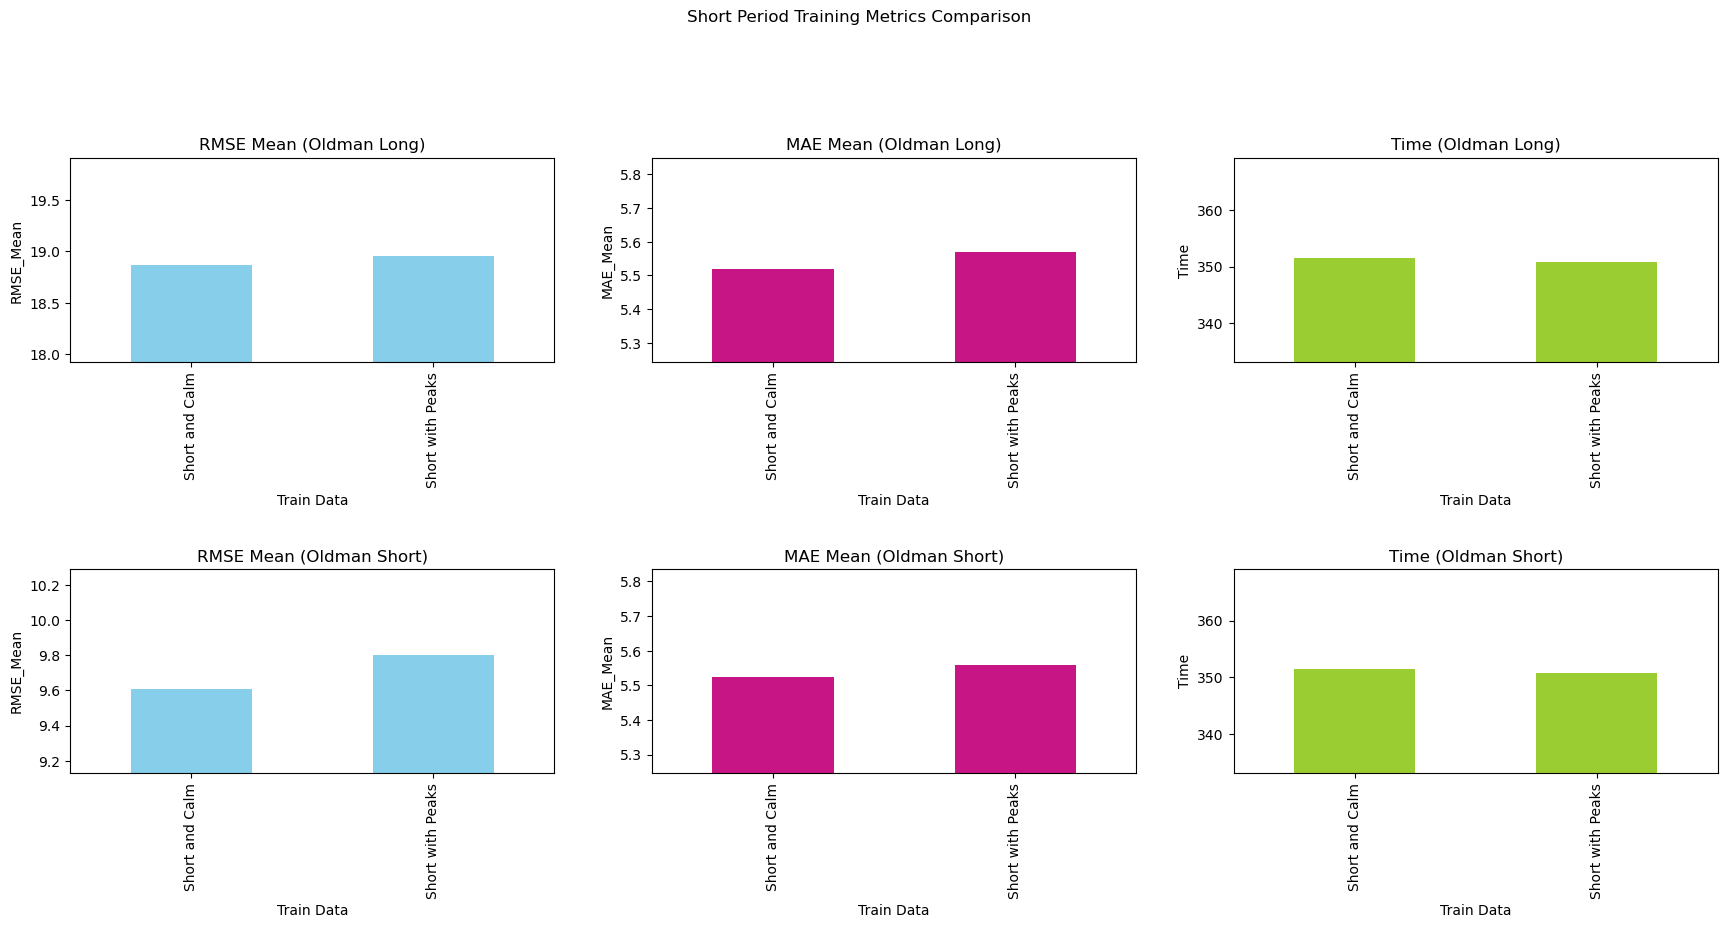
\includegraphics[width=.8\textwidth]{figures/time_series_analysis/comparison/short_period.png}
    \captionsetup{width=.8\textwidth}
    \caption{Comparison of metrics for the test case of short periods}
    \label{fig:enter-label}
\end{figure}

The second comparison is between training time series of long periods. Logical relationships are also derived in this case, where the posterior sampled from the long time series with peaks, where anomalies occur now and then, delivers better performance. Having appropriate amounts of anomalies in the training data set, the posterior can resemble the regularity of presence in terms of patterns of anomalies, while it keeps the model robust and accurate in predicting calm phases. This balance helps the model to better generalize and adapt to unexpected variations in the data.
\begin{figure}[H]
    \centering
    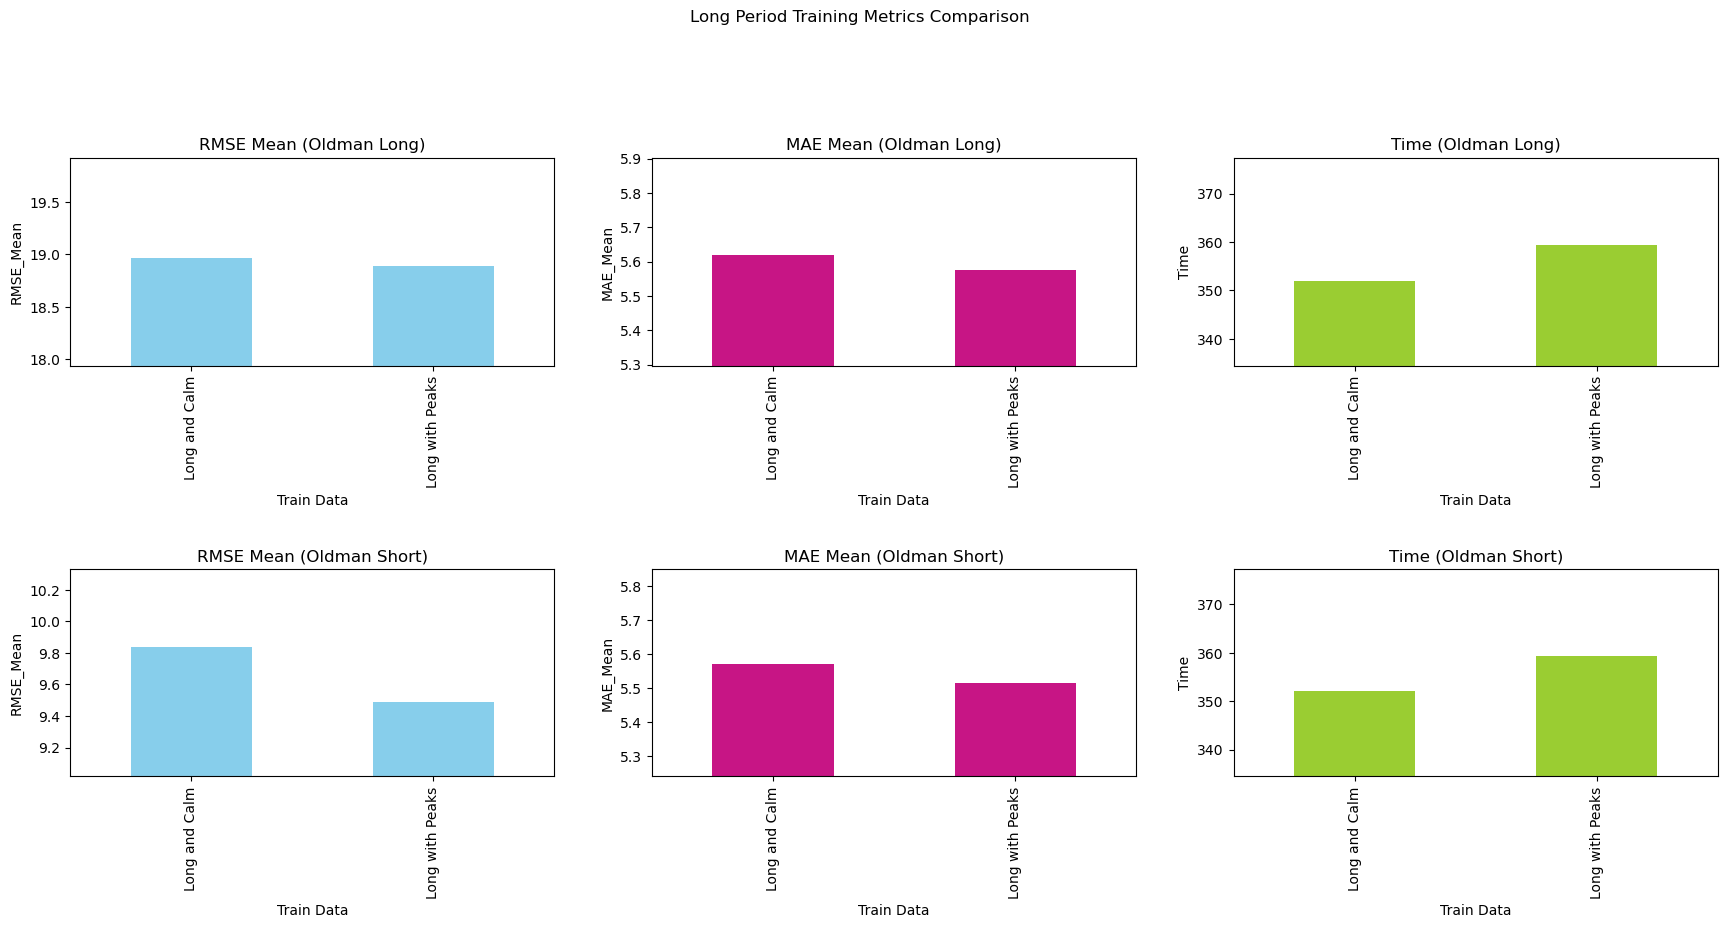
\includegraphics[width=.8\textwidth]{figures/time_series_analysis/comparison/long_period.png}
    \captionsetup{width=.8\textwidth}
    \caption{Comparison of metrics for the test case of long periods}
    \label{fig:enter-label}
\end{figure}

For the third comparison, we focus on periods with peaks. A short time series with peaks is compared with a long time series with peaks so that the importance of the training period length is focused. From the results, we can observe that the long training time series generally delivers a better performance than the short training time series. This observation is reasonable, since the long training time series contains more anomalies over time, allowing the posterior to learn and adapt to the pattern in the process of sampling. A longer period for training time series here means that the posterior is exposed to more anomalies, allowing the adaption to take place, thus potentially resulting in better accuracy scores.

\begin{figure}[H]
    \centering
    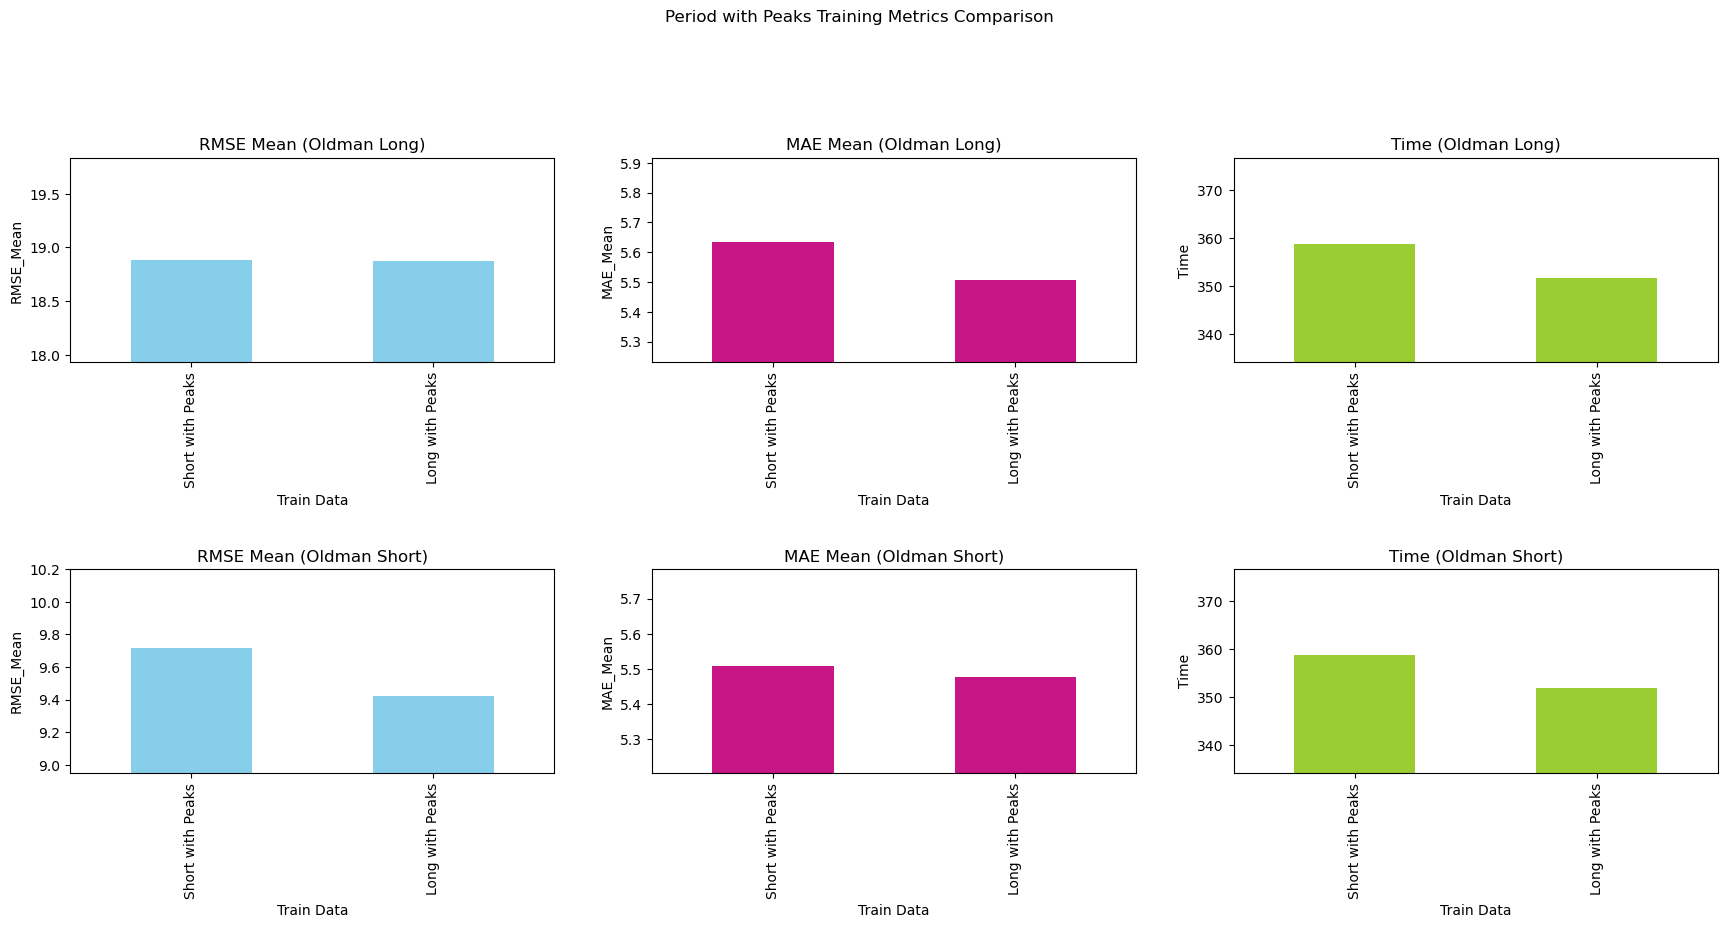
\includegraphics[width=.8\textwidth]{figures/time_series_analysis/comparison/period_with_peaks.png}
    \captionsetup{width=.8\textwidth}
    \caption{Comparison of metrics for the test case of periods with peaks}
    \label{fig:enter-label}
\end{figure}

The fourth comparison is more generalized. Time series between 1997 and 2003 of both Banff and Oldman basins, which contain both peak and calm phases, are used to generate posteriors, where they are then tested on two testing data frames selected from both basins. For the test data frame from the Oldman basin, the posterior sampled from the Oldman basin achieved a better accuracy score than the posterior sampled from the Banff basin. This is logical because the sampling process adapts itself to the behavior of the Oldman basin. However, the posterior sample from the Oldman basin also performs better for the test data frame from the Banff basin than the posterior sampled from the Banff basin. This could be due to the same reason as mentioned in the first comparison since anomalies are still. 
Being trained on the Oldman basin instead of the Banff basin, the posterior is more accustomed to the calm periods, which still constitutes the majority part of the time series from the Banff basin. Therefore, training on the Oldman basin is overall a better choice for general Bayesian inference results.
\begin{figure}[H]
    \centering
    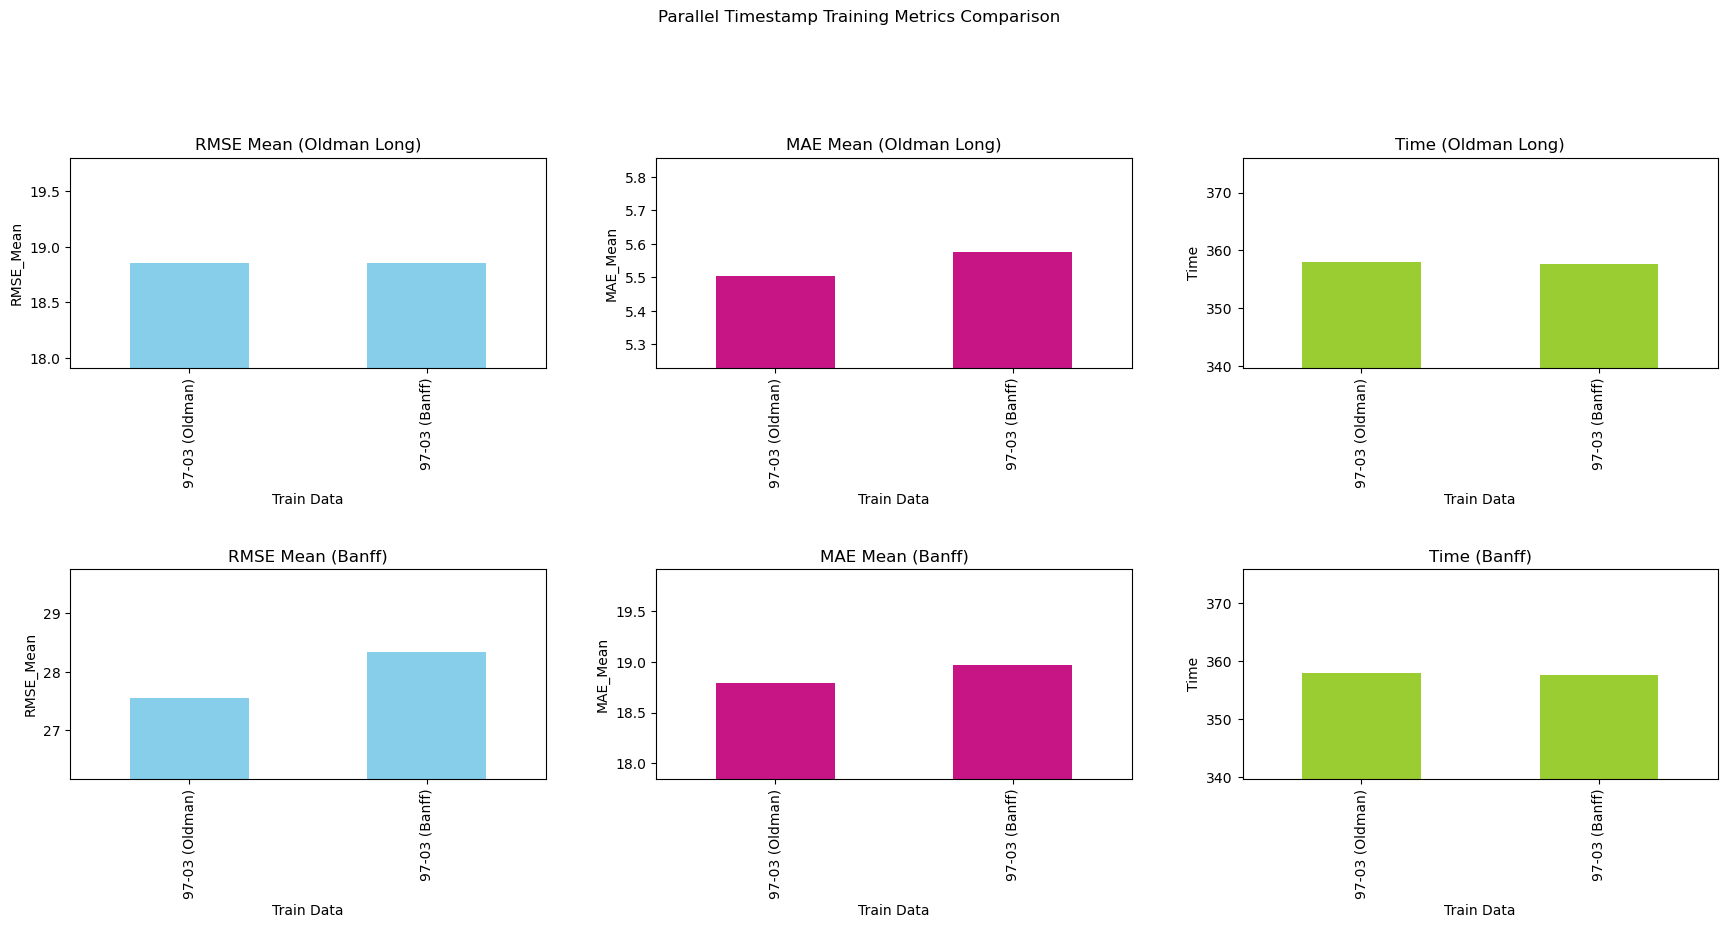
\includegraphics[width=.8\textwidth]{figures/time_series_analysis/comparison/parallel_timestamp.png}
    \captionsetup{width=.8\textwidth}
    \caption{Comparison of metrics for the test case of periods from different basins}
    \label{fig:enter-label}
\end{figure}

The spin-up phase is investigated for the last comparison. The efficiency is more optimized for the models with shorter spin-up phases, which is logical since spin-up phases require model executions and simulations as well. For the accuracy metrics, on the other hand, the results show a certain complexity for analysis. Testing the sampled posterior on the short test data frame results in a proportional relationship, in which shorter spin-up phases result in better accuracy scores. This might be because longer spin-up phases consider too much historical data, which might potentially be a disturbing factor for the Bayesian inference. For the long test data frame, there is no pattern that can be distinguished regarding the relationship between the accuracy score and the spin-up length. Since the longer data frame contains more anomalies, the behavior of the posterior sampling can be unpredictable. Therefore, the spin-up length may not consistently influence the accuracy score.

\begin{figure}[H]
    \centering
    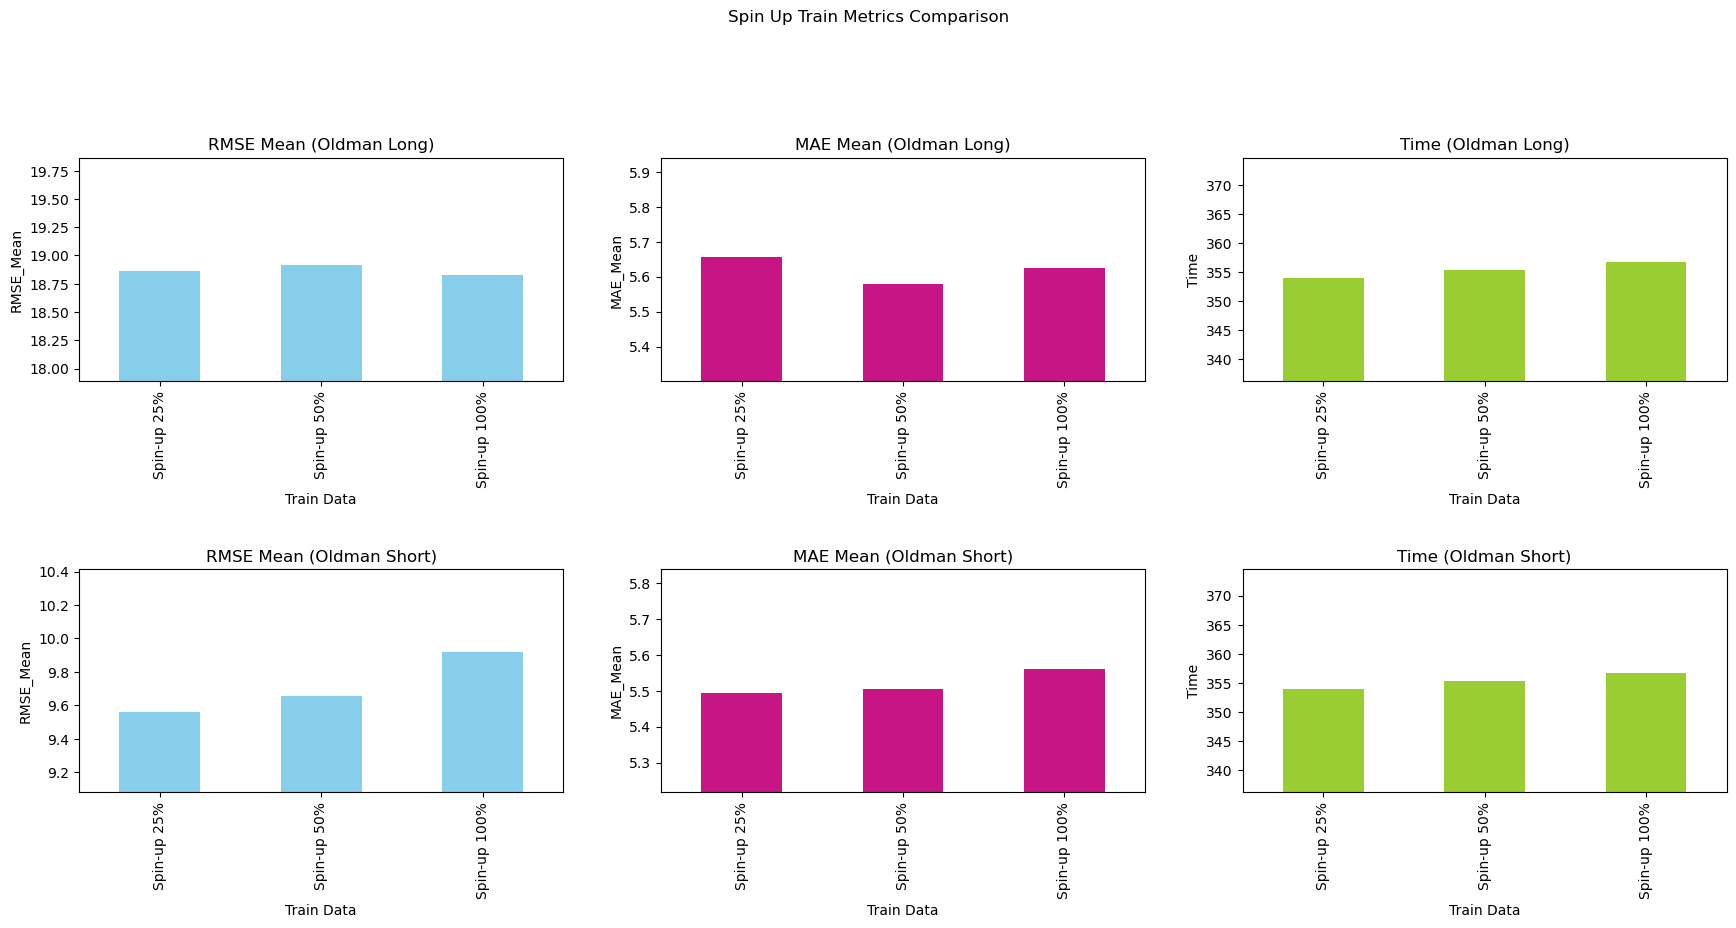
\includegraphics[width=.8\textwidth]{figures/time_series_analysis/comparison/spin_up.png}
    \captionsetup{width=.8\textwidth}
    \caption{Comparison of metrics for the observation of spin-up length}
    \label{fig:enter-label}
\end{figure}

In conclusion, focusing on sampling from data where more peaks are present allows the Markov chain Monte Carlo algorithm to perform more precise predictions for anomalies, whereas concentrating on sampling from data that are calmer and contain fewer anomalies allows the Markov chain Monte Carlo algorithm to perform generally better forecasts in terms of accuracy metrics. A selection of training data that balances both aspects is crucial for optimal inferred results.
